% Options for packages loaded elsewhere
\PassOptionsToPackage{unicode}{hyperref}
\PassOptionsToPackage{hyphens}{url}
%
\documentclass[
]{article}
\usepackage{amsmath,amssymb}
\usepackage{iftex}
\ifPDFTeX
  \usepackage[T1]{fontenc}
  \usepackage[utf8]{inputenc}
  \usepackage{textcomp} % provide euro and other symbols
\else % if luatex or xetex
  \usepackage{unicode-math} % this also loads fontspec
  \defaultfontfeatures{Scale=MatchLowercase}
  \defaultfontfeatures[\rmfamily]{Ligatures=TeX,Scale=1}
\fi
\usepackage{lmodern}
\ifPDFTeX\else
  % xetex/luatex font selection
\fi
% Use upquote if available, for straight quotes in verbatim environments
\IfFileExists{upquote.sty}{\usepackage{upquote}}{}
\IfFileExists{microtype.sty}{% use microtype if available
  \usepackage[]{microtype}
  \UseMicrotypeSet[protrusion]{basicmath} % disable protrusion for tt fonts
}{}
\makeatletter
\@ifundefined{KOMAClassName}{% if non-KOMA class
  \IfFileExists{parskip.sty}{%
    \usepackage{parskip}
  }{% else
    \setlength{\parindent}{0pt}
    \setlength{\parskip}{6pt plus 2pt minus 1pt}}
}{% if KOMA class
  \KOMAoptions{parskip=half}}
\makeatother
\usepackage{xcolor}
\usepackage[margin=1in]{geometry}
\usepackage{color}
\usepackage{fancyvrb}
\newcommand{\VerbBar}{|}
\newcommand{\VERB}{\Verb[commandchars=\\\{\}]}
\DefineVerbatimEnvironment{Highlighting}{Verbatim}{commandchars=\\\{\}}
% Add ',fontsize=\small' for more characters per line
\usepackage{framed}
\definecolor{shadecolor}{RGB}{248,248,248}
\newenvironment{Shaded}{\begin{snugshade}}{\end{snugshade}}
\newcommand{\AlertTok}[1]{\textcolor[rgb]{0.94,0.16,0.16}{#1}}
\newcommand{\AnnotationTok}[1]{\textcolor[rgb]{0.56,0.35,0.01}{\textbf{\textit{#1}}}}
\newcommand{\AttributeTok}[1]{\textcolor[rgb]{0.13,0.29,0.53}{#1}}
\newcommand{\BaseNTok}[1]{\textcolor[rgb]{0.00,0.00,0.81}{#1}}
\newcommand{\BuiltInTok}[1]{#1}
\newcommand{\CharTok}[1]{\textcolor[rgb]{0.31,0.60,0.02}{#1}}
\newcommand{\CommentTok}[1]{\textcolor[rgb]{0.56,0.35,0.01}{\textit{#1}}}
\newcommand{\CommentVarTok}[1]{\textcolor[rgb]{0.56,0.35,0.01}{\textbf{\textit{#1}}}}
\newcommand{\ConstantTok}[1]{\textcolor[rgb]{0.56,0.35,0.01}{#1}}
\newcommand{\ControlFlowTok}[1]{\textcolor[rgb]{0.13,0.29,0.53}{\textbf{#1}}}
\newcommand{\DataTypeTok}[1]{\textcolor[rgb]{0.13,0.29,0.53}{#1}}
\newcommand{\DecValTok}[1]{\textcolor[rgb]{0.00,0.00,0.81}{#1}}
\newcommand{\DocumentationTok}[1]{\textcolor[rgb]{0.56,0.35,0.01}{\textbf{\textit{#1}}}}
\newcommand{\ErrorTok}[1]{\textcolor[rgb]{0.64,0.00,0.00}{\textbf{#1}}}
\newcommand{\ExtensionTok}[1]{#1}
\newcommand{\FloatTok}[1]{\textcolor[rgb]{0.00,0.00,0.81}{#1}}
\newcommand{\FunctionTok}[1]{\textcolor[rgb]{0.13,0.29,0.53}{\textbf{#1}}}
\newcommand{\ImportTok}[1]{#1}
\newcommand{\InformationTok}[1]{\textcolor[rgb]{0.56,0.35,0.01}{\textbf{\textit{#1}}}}
\newcommand{\KeywordTok}[1]{\textcolor[rgb]{0.13,0.29,0.53}{\textbf{#1}}}
\newcommand{\NormalTok}[1]{#1}
\newcommand{\OperatorTok}[1]{\textcolor[rgb]{0.81,0.36,0.00}{\textbf{#1}}}
\newcommand{\OtherTok}[1]{\textcolor[rgb]{0.56,0.35,0.01}{#1}}
\newcommand{\PreprocessorTok}[1]{\textcolor[rgb]{0.56,0.35,0.01}{\textit{#1}}}
\newcommand{\RegionMarkerTok}[1]{#1}
\newcommand{\SpecialCharTok}[1]{\textcolor[rgb]{0.81,0.36,0.00}{\textbf{#1}}}
\newcommand{\SpecialStringTok}[1]{\textcolor[rgb]{0.31,0.60,0.02}{#1}}
\newcommand{\StringTok}[1]{\textcolor[rgb]{0.31,0.60,0.02}{#1}}
\newcommand{\VariableTok}[1]{\textcolor[rgb]{0.00,0.00,0.00}{#1}}
\newcommand{\VerbatimStringTok}[1]{\textcolor[rgb]{0.31,0.60,0.02}{#1}}
\newcommand{\WarningTok}[1]{\textcolor[rgb]{0.56,0.35,0.01}{\textbf{\textit{#1}}}}
\usepackage{longtable,booktabs,array}
\usepackage{calc} % for calculating minipage widths
% Correct order of tables after \paragraph or \subparagraph
\usepackage{etoolbox}
\makeatletter
\patchcmd\longtable{\par}{\if@noskipsec\mbox{}\fi\par}{}{}
\makeatother
% Allow footnotes in longtable head/foot
\IfFileExists{footnotehyper.sty}{\usepackage{footnotehyper}}{\usepackage{footnote}}
\makesavenoteenv{longtable}
\usepackage{graphicx}
\makeatletter
\def\maxwidth{\ifdim\Gin@nat@width>\linewidth\linewidth\else\Gin@nat@width\fi}
\def\maxheight{\ifdim\Gin@nat@height>\textheight\textheight\else\Gin@nat@height\fi}
\makeatother
% Scale images if necessary, so that they will not overflow the page
% margins by default, and it is still possible to overwrite the defaults
% using explicit options in \includegraphics[width, height, ...]{}
\setkeys{Gin}{width=\maxwidth,height=\maxheight,keepaspectratio}
% Set default figure placement to htbp
\makeatletter
\def\fps@figure{htbp}
\makeatother
\setlength{\emergencystretch}{3em} % prevent overfull lines
\providecommand{\tightlist}{%
  \setlength{\itemsep}{0pt}\setlength{\parskip}{0pt}}
\setcounter{secnumdepth}{-\maxdimen} % remove section numbering
\usepackage{booktabs}
\usepackage{longtable}
\usepackage{array}
\usepackage{multirow}
\usepackage{wrapfig}
\usepackage{float}
\usepackage{colortbl}
\usepackage{pdflscape}
\usepackage{tabu}
\usepackage{threeparttable}
\usepackage{threeparttablex}
\usepackage[normalem]{ulem}
\usepackage{makecell}
\usepackage{xcolor}
\ifLuaTeX
  \usepackage{selnolig}  % disable illegal ligatures
\fi
\IfFileExists{bookmark.sty}{\usepackage{bookmark}}{\usepackage{hyperref}}
\IfFileExists{xurl.sty}{\usepackage{xurl}}{} % add URL line breaks if available
\urlstyle{same}
\hypersetup{
  pdftitle={EL VOTO AUTONÓMICO EN LA COMARCA DE LA SAFOR ( VALENCIA )},
  pdfauthor={Tomàs Ferrandis Moscardó},
  hidelinks,
  pdfcreator={LaTeX via pandoc}}

\title{EL VOTO AUTONÓMICO EN LA COMARCA DE LA SAFOR ( VALENCIA )}
\author{Tomàs Ferrandis Moscardó}
\date{2024-01-26}

\begin{document}
\maketitle

{
\setcounter{tocdepth}{2}
\tableofcontents
}
\hypertarget{obtenciuxf3n-y-representaciuxf3n-de-algunos-valores-estaduxedsticos.}{%
\section{OBTENCIÓN Y REPRESENTACIÓN DE ALGUNOS VALORES
ESTADÍSTICOS.}\label{obtenciuxf3n-y-representaciuxf3n-de-algunos-valores-estaduxedsticos.}}

A continuación veremos un sencillo ejemplo de uso de R Markdown en el
que, a partir de un fichero \emph{csv} con resultados electorales,
crearemos y manipularemos objetos data.frame para obtener algunas
medidas de tendencia central y dispersión que representaremos en tablas
y gráficos.

\hypertarget{obtenciuxf3n-de-los-datos}{%
\subsection{OBTENCIÓN DE LOS DATOS}\label{obtenciuxf3n-de-los-datos}}

\hypertarget{resultados-de-todas-las-elecciones-y-convocatorias-a-nivel-de-agregaciuxf3n-comarcal.-caso-de-la-safor.}{%
\subsubsection{Resultados de todas las elecciones y convocatorias a
nivel de agregación comarcal. Caso de La
Safor.}\label{resultados-de-todas-las-elecciones-y-convocatorias-a-nivel-de-agregaciuxf3n-comarcal.-caso-de-la-safor.}}

A partir de la base de datos de ARGOS descargamos el resumen de
resultados electorales en las distintas convocatorias y procesos
electorales en un fichero CSV.

\begin{Shaded}
\begin{Highlighting}[]
\NormalTok{df1}\OtherTok{\textless{}{-}}\FunctionTok{read.csv}\NormalTok{(}\StringTok{"CSV/SAFOR.csv"}\NormalTok{,}\AttributeTok{header=}\ConstantTok{TRUE}\NormalTok{, }\AttributeTok{sep=}\StringTok{","}\NormalTok{,}\AttributeTok{quote=}\StringTok{"}\SpecialCharTok{\textbackslash{}"}\StringTok{\textquotesingle{}"}\NormalTok{, }\AttributeTok{dec=}\StringTok{","}\NormalTok{,}\AttributeTok{fill=}\ConstantTok{TRUE}\NormalTok{,}
              \AttributeTok{comment.char =} \StringTok{""}\NormalTok{)}
\CommentTok{\#View(df1) \# Para ver en consola}
\end{Highlighting}
\end{Shaded}

\hypertarget{filtramos-por-elecciones-autonuxf3micas.}{%
\subsubsection{Filtramos por elecciones
autonómicas.}\label{filtramos-por-elecciones-autonuxf3micas.}}

Asumimos como universo o población el conjunto de todas las elecciones
autonómicas.

\begin{Shaded}
\begin{Highlighting}[]
\NormalTok{df\_autonomicas}\OtherTok{\textless{}{-}}\NormalTok{df1 }\SpecialCharTok{\%\textgreater{}\%} \FunctionTok{filter}\NormalTok{(}\FunctionTok{str\_detect}\NormalTok{(df1}\SpecialCharTok{$}\NormalTok{Elecció,}\StringTok{"A{-}"}\NormalTok{))}
\CommentTok{\# Vemos las 10 primeras lineas de ejemplo}
\FunctionTok{head}\NormalTok{(df\_autonomicas)}
\end{Highlighting}
\end{Shaded}

\begin{verbatim}
##   Elecció   Cens A.Cand.    PP  PSPV COMPROMÍS  VOX PODEMOS    Cs EUPV RESTA
## 1  A-2023 124367   86496 28245 25559     19953 8282    2234   591   NA  1859
## 2  A-2019 121181   89534 17325 19867     23504 7666    5917 12394   NA  2861
## 3  A-2015 121362   90086 26377 18226     24789  207    6845  7668 3129  2845
## 4  A-2011 120877   92475 47413 25159     12366   NA      NA    NA 3323  4214
## 5  A-2007 119109   90705 46558 29321     11050   NA      NA    NA   NA  3776
## 6  A-2003 116160   90337 41220 31192     10891   NA      NA    NA 3145  3889
\end{verbatim}

\hypertarget{tratamiento-de-los-na}{%
\subsubsection{Tratamiento de los NA}\label{tratamiento-de-los-na}}

En nuestro caso los NA se deben a la ausencia de resultados por no
haberse presentado la fuerza política en una conveocatoria o haberse
integrado en una coalición electoral. Entendemos que el valor que debe
sustituir NA para poder realizar cálculos estadísticos de forma correcta
y sin errores de computación es el 0. Podríamos recorrer solo las
columnas de partidos pero lo simplificamos y aplicamos la sustitución NA
-\textgreater{} 0 en todo el data frame.

\begin{Shaded}
\begin{Highlighting}[]
\NormalTok{df\_autonomicas[}\FunctionTok{is.na}\NormalTok{(df\_autonomicas)]}\OtherTok{\textless{}{-}}\DecValTok{0}
\NormalTok{knitr}\SpecialCharTok{::}\FunctionTok{kable}\NormalTok{(df\_autonomicas, }\AttributeTok{caption =} \StringTok{"ELECCIONES AUTONÓMICAS EN LA SAFOR"}\NormalTok{)}
\end{Highlighting}
\end{Shaded}

\begin{longtable}[]{@{}
  >{\raggedright\arraybackslash}p{(\columnwidth - 20\tabcolsep) * \real{0.1067}}
  >{\raggedleft\arraybackslash}p{(\columnwidth - 20\tabcolsep) * \real{0.0933}}
  >{\raggedleft\arraybackslash}p{(\columnwidth - 20\tabcolsep) * \real{0.1067}}
  >{\raggedleft\arraybackslash}p{(\columnwidth - 20\tabcolsep) * \real{0.0800}}
  >{\raggedleft\arraybackslash}p{(\columnwidth - 20\tabcolsep) * \real{0.0800}}
  >{\raggedleft\arraybackslash}p{(\columnwidth - 20\tabcolsep) * \real{0.1333}}
  >{\raggedleft\arraybackslash}p{(\columnwidth - 20\tabcolsep) * \real{0.0667}}
  >{\raggedleft\arraybackslash}p{(\columnwidth - 20\tabcolsep) * \real{0.1067}}
  >{\raggedleft\arraybackslash}p{(\columnwidth - 20\tabcolsep) * \real{0.0800}}
  >{\raggedleft\arraybackslash}p{(\columnwidth - 20\tabcolsep) * \real{0.0667}}
  >{\raggedleft\arraybackslash}p{(\columnwidth - 20\tabcolsep) * \real{0.0800}}@{}}
\caption{ELECCIONES AUTONÓMICAS EN LA SAFOR}\tabularnewline
\toprule\noalign{}
\begin{minipage}[b]{\linewidth}\raggedright
Elecció
\end{minipage} & \begin{minipage}[b]{\linewidth}\raggedleft
Cens
\end{minipage} & \begin{minipage}[b]{\linewidth}\raggedleft
A.Cand.
\end{minipage} & \begin{minipage}[b]{\linewidth}\raggedleft
PP
\end{minipage} & \begin{minipage}[b]{\linewidth}\raggedleft
PSPV
\end{minipage} & \begin{minipage}[b]{\linewidth}\raggedleft
COMPROMÍS
\end{minipage} & \begin{minipage}[b]{\linewidth}\raggedleft
VOX
\end{minipage} & \begin{minipage}[b]{\linewidth}\raggedleft
PODEMOS
\end{minipage} & \begin{minipage}[b]{\linewidth}\raggedleft
Cs
\end{minipage} & \begin{minipage}[b]{\linewidth}\raggedleft
EUPV
\end{minipage} & \begin{minipage}[b]{\linewidth}\raggedleft
RESTA
\end{minipage} \\
\midrule\noalign{}
\endfirsthead
\toprule\noalign{}
\begin{minipage}[b]{\linewidth}\raggedright
Elecció
\end{minipage} & \begin{minipage}[b]{\linewidth}\raggedleft
Cens
\end{minipage} & \begin{minipage}[b]{\linewidth}\raggedleft
A.Cand.
\end{minipage} & \begin{minipage}[b]{\linewidth}\raggedleft
PP
\end{minipage} & \begin{minipage}[b]{\linewidth}\raggedleft
PSPV
\end{minipage} & \begin{minipage}[b]{\linewidth}\raggedleft
COMPROMÍS
\end{minipage} & \begin{minipage}[b]{\linewidth}\raggedleft
VOX
\end{minipage} & \begin{minipage}[b]{\linewidth}\raggedleft
PODEMOS
\end{minipage} & \begin{minipage}[b]{\linewidth}\raggedleft
Cs
\end{minipage} & \begin{minipage}[b]{\linewidth}\raggedleft
EUPV
\end{minipage} & \begin{minipage}[b]{\linewidth}\raggedleft
RESTA
\end{minipage} \\
\midrule\noalign{}
\endhead
\bottomrule\noalign{}
\endlastfoot
A-2023 & 124367 & 86496 & 28245 & 25559 & 19953 & 8282 & 2234 & 591 & 0
& 1859 \\
A-2019 & 121181 & 89534 & 17325 & 19867 & 23504 & 7666 & 5917 & 12394 &
0 & 2861 \\
A-2015 & 121362 & 90086 & 26377 & 18226 & 24789 & 207 & 6845 & 7668 &
3129 & 2845 \\
A-2011 & 120877 & 92475 & 47413 & 25159 & 12366 & 0 & 0 & 0 & 3323 &
4214 \\
A-2007 & 119109 & 90705 & 46558 & 29321 & 11050 & 0 & 0 & 0 & 0 &
3776 \\
A-2003 & 116160 & 90337 & 41220 & 31192 & 10891 & 0 & 0 & 0 & 3145 &
3889 \\
A-1999 & 117654 & 87007 & 40176 & 27696 & 9066 & 0 & 0 & 0 & 3782 &
6287 \\
A-1995 & 108888 & 86600 & 32374 & 29415 & 7600 & 0 & 0 & 0 & 7503 &
9708 \\
A-1991 & 102923 & 78619 & 19181 & 30884 & 7998 & 0 & 0 & 0 & 5313 &
15243 \\
A-1987 & 97022 & 75807 & 17142 & 28744 & 0 & 0 & 0 & 0 & 9042 & 20879 \\
A-1983 & 94401 & 72681 & 22015 & 30781 & 5823 & 0 & 0 & 0 & 5815 &
8247 \\
\end{longtable}

\hypertarget{creamos-un-vector-con-las-candidaturas.}{%
\subsection{Creamos un vector con las
candidaturas.}\label{creamos-un-vector-con-las-candidaturas.}}

\begin{Shaded}
\begin{Highlighting}[]
\CommentTok{\# Recogemos los nombres de columnas a partir de la 4ª}
\NormalTok{partits}\OtherTok{\textless{}{-}}\FunctionTok{names}\NormalTok{(df1[}\DecValTok{4}\SpecialCharTok{:}\FunctionTok{length}\NormalTok{(df1)])}

\CommentTok{\# O directamente, para nuestro caso}
\CommentTok{\#partits\textless{}{-}c("PP","PSPV","COMPROMÍS","VOX","PODEMOS","Cs","EUPV","RESTA")}
\end{Highlighting}
\end{Shaded}

\hypertarget{calculamos-algunos-valores-de-medidas-tendencia-central-y-dispersiuxf3n}{%
\subsection{Calculamos algunos valores de medidas tendencia central y
dispersión}\label{calculamos-algunos-valores-de-medidas-tendencia-central-y-dispersiuxf3n}}

1.- Media o promedio 2.- Máximos 3.- Míninos 4.- Rango de variación

\begin{Shaded}
\begin{Highlighting}[]
\NormalTok{mitjana}\OtherTok{\textless{}{-}}\FunctionTok{summarise\_at}\NormalTok{(df\_autonomicas,partits,mean)}
\NormalTok{maxims}\OtherTok{\textless{}{-}}\FunctionTok{summarise\_at}\NormalTok{(df\_autonomicas,partits,max)}
\NormalTok{minims}\OtherTok{\textless{}{-}}\FunctionTok{summarise\_at}\NormalTok{(df\_autonomicas,partits,}\SpecialCharTok{\textasciitilde{}}\FunctionTok{min}\NormalTok{(.[. }\SpecialCharTok{!=} \DecValTok{0}\NormalTok{])) }\CommentTok{\#Descartamos los 0}
\NormalTok{rangodevariacion}\OtherTok{\textless{}{-}}\NormalTok{maxims }\SpecialCharTok{{-}}\NormalTok{ minims}

\CommentTok{\#Creamos un data frame. cada vector anterior será una columna}
\NormalTok{df\_resultats}\OtherTok{\textless{}{-}}\FunctionTok{rbind}\NormalTok{(mitjana)}
\NormalTok{df\_resultats}\OtherTok{\textless{}{-}}\FunctionTok{rbind}\NormalTok{(df\_resultats,maxims)}
\NormalTok{df\_resultats}\OtherTok{\textless{}{-}}\FunctionTok{rbind}\NormalTok{(df\_resultats,minims)}
\NormalTok{df\_resultats}\OtherTok{\textless{}{-}}\FunctionTok{rbind}\NormalTok{(df\_resultats,rangodevariacion)}
\CommentTok{\#Redondeamos los valores a enteros ( son votos) }
\NormalTok{df\_resultats}\OtherTok{\textless{}{-}}\NormalTok{df\_resultats }\SpecialCharTok{\%\textgreater{}\%} \FunctionTok{mutate\_at}\NormalTok{(partits, as.integer)}

\CommentTok{\#Añadimos al final del data frame una columna con el nombre del "cálculo"}
\NormalTok{df\_resultats}\OtherTok{\textless{}{-}}\FunctionTok{cbind}\NormalTok{(df\_resultats,ESTADÍSTICA}\OtherTok{=}\FunctionTok{c}\NormalTok{(}\StringTok{"MEDIA"}\NormalTok{,}\StringTok{"MÁXIMO"}\NormalTok{,}\StringTok{"MÍNIMO"}\NormalTok{,}\StringTok{"RANGO"}\NormalTok{))}
\CommentTok{\# la resituamos en la posición 1 ( estética)}
\NormalTok{df\_resultats}\OtherTok{\textless{}{-}}\NormalTok{df\_resultats }\SpecialCharTok{\%\textgreater{}\%} \FunctionTok{select}\NormalTok{(}\StringTok{"ESTADÍSTICA"}\NormalTok{,}\FunctionTok{everything}\NormalTok{())}

\CommentTok{\#Imprimimos en Markdown una tabla con los resultados}
\NormalTok{knitr}\SpecialCharTok{::}\FunctionTok{kable}\NormalTok{(df\_resultats, }\AttributeTok{caption =} \StringTok{"ESTADÍSTICA SAFOR"}\NormalTok{)}
\end{Highlighting}
\end{Shaded}

\begin{longtable}[]{@{}
  >{\raggedright\arraybackslash}p{(\columnwidth - 16\tabcolsep) * \real{0.1875}}
  >{\raggedleft\arraybackslash}p{(\columnwidth - 16\tabcolsep) * \real{0.0938}}
  >{\raggedleft\arraybackslash}p{(\columnwidth - 16\tabcolsep) * \real{0.0938}}
  >{\raggedleft\arraybackslash}p{(\columnwidth - 16\tabcolsep) * \real{0.1562}}
  >{\raggedleft\arraybackslash}p{(\columnwidth - 16\tabcolsep) * \real{0.0781}}
  >{\raggedleft\arraybackslash}p{(\columnwidth - 16\tabcolsep) * \real{0.1250}}
  >{\raggedleft\arraybackslash}p{(\columnwidth - 16\tabcolsep) * \real{0.0938}}
  >{\raggedleft\arraybackslash}p{(\columnwidth - 16\tabcolsep) * \real{0.0781}}
  >{\raggedleft\arraybackslash}p{(\columnwidth - 16\tabcolsep) * \real{0.0938}}@{}}
\caption{ESTADÍSTICA SAFOR}\tabularnewline
\toprule\noalign{}
\begin{minipage}[b]{\linewidth}\raggedright
ESTADÍSTICA
\end{minipage} & \begin{minipage}[b]{\linewidth}\raggedleft
PP
\end{minipage} & \begin{minipage}[b]{\linewidth}\raggedleft
PSPV
\end{minipage} & \begin{minipage}[b]{\linewidth}\raggedleft
COMPROMÍS
\end{minipage} & \begin{minipage}[b]{\linewidth}\raggedleft
VOX
\end{minipage} & \begin{minipage}[b]{\linewidth}\raggedleft
PODEMOS
\end{minipage} & \begin{minipage}[b]{\linewidth}\raggedleft
Cs
\end{minipage} & \begin{minipage}[b]{\linewidth}\raggedleft
EUPV
\end{minipage} & \begin{minipage}[b]{\linewidth}\raggedleft
RESTA
\end{minipage} \\
\midrule\noalign{}
\endfirsthead
\toprule\noalign{}
\begin{minipage}[b]{\linewidth}\raggedright
ESTADÍSTICA
\end{minipage} & \begin{minipage}[b]{\linewidth}\raggedleft
PP
\end{minipage} & \begin{minipage}[b]{\linewidth}\raggedleft
PSPV
\end{minipage} & \begin{minipage}[b]{\linewidth}\raggedleft
COMPROMÍS
\end{minipage} & \begin{minipage}[b]{\linewidth}\raggedleft
VOX
\end{minipage} & \begin{minipage}[b]{\linewidth}\raggedleft
PODEMOS
\end{minipage} & \begin{minipage}[b]{\linewidth}\raggedleft
Cs
\end{minipage} & \begin{minipage}[b]{\linewidth}\raggedleft
EUPV
\end{minipage} & \begin{minipage}[b]{\linewidth}\raggedleft
RESTA
\end{minipage} \\
\midrule\noalign{}
\endhead
\bottomrule\noalign{}
\endlastfoot
MEDIA & 30729 & 26985 & 12094 & 1468 & 1363 & 1877 & 3732 & 7255 \\
MÁXIMO & 47413 & 31192 & 24789 & 8282 & 6845 & 12394 & 9042 & 20879 \\
MÍNIMO & 17142 & 18226 & 5823 & 207 & 2234 & 591 & 3129 & 1859 \\
RANGO & 30271 & 12966 & 18966 & 8075 & 4611 & 11803 & 5913 & 19020 \\
\end{longtable}

\hypertarget{gruxe1ficos}{%
\subsection{GRÁFICOS}\label{gruxe1ficos}}

Vemos a continuación los gráficos y tablas de daraso a nivel de
agregación de candidatura.

\begin{Shaded}
\begin{Highlighting}[]
\CommentTok{\# Recorremos las columnas del data frame correspondientes a candidaturas ( \textgreater{}2)}
\CommentTok{\# Creamos un data frame en cada iteración}
\ControlFlowTok{for}\NormalTok{ ( i }\ControlFlowTok{in} \DecValTok{2}\SpecialCharTok{:}\FunctionTok{length}\NormalTok{(df\_resultats))\{}
\NormalTok{     df\_estPartit}\OtherTok{\textless{}{-}} \FunctionTok{data.frame}\NormalTok{(}
\NormalTok{         ESTADÍSTICA}\OtherTok{=}\NormalTok{df\_resultats}\SpecialCharTok{$}\NormalTok{ESTADÍSTICA,}
         \AttributeTok{VALORS=}\NormalTok{df\_resultats[,i],}
         \AttributeTok{PARTIT=}\FunctionTok{colnames}\NormalTok{(df\_resultats[i])}
\NormalTok{     )}

\CommentTok{\# EN UN GRAFICO}
\FunctionTok{barplot}\NormalTok{(df\_estPartit}\SpecialCharTok{$}\NormalTok{VALORS, }
        \AttributeTok{main=}\FunctionTok{paste}\NormalTok{(}\StringTok{"Valores estadísticos de"}\NormalTok{,df\_estPartit}\SpecialCharTok{$}\NormalTok{PARTIT[}\DecValTok{1}\NormalTok{]),}
        \AttributeTok{names.arg=}\NormalTok{df\_estPartit}\SpecialCharTok{$}\NormalTok{ESTADÍSTICA,}
        \AttributeTok{col=}\FunctionTok{c}\NormalTok{(}\StringTok{"\#5fe10b"}\NormalTok{,}\StringTok{"red"}\NormalTok{,}\StringTok{"\#48b7f7"}\NormalTok{,}\StringTok{"\#ede12e"}\NormalTok{),}
        \AttributeTok{ylab=}\StringTok{"VOTOS"}\NormalTok{)}


\CommentTok{\# EN UNA TABLA}
\CommentTok{\#Quitamos la columna que repite el nombre ( estético), lo guardamos antes}
\NormalTok{candidatura}\OtherTok{\textless{}{-}}\NormalTok{df\_estPartit}\SpecialCharTok{$}\NormalTok{PARTIT[}\DecValTok{1}\NormalTok{]}
\NormalTok{df\_estPartit }\OtherTok{\textless{}{-}}\NormalTok{ df\_estPartit[, }\SpecialCharTok{!}\NormalTok{(}\FunctionTok{names}\NormalTok{(df\_estPartit) }\SpecialCharTok{\%in\%} \StringTok{"PARTIT"}\NormalTok{)]}
\NormalTok{knitr}\SpecialCharTok{::}\FunctionTok{kable}\NormalTok{(df\_estPartit, }\AttributeTok{caption =} \FunctionTok{paste}\NormalTok{( }\StringTok{"ESTADÍSTICA SAFOR"}\NormalTok{, }
\NormalTok{                        candidatura )) }\SpecialCharTok{\%\textgreater{}\%} \FunctionTok{print}\NormalTok{()}


\NormalTok{\}}
\end{Highlighting}
\end{Shaded}

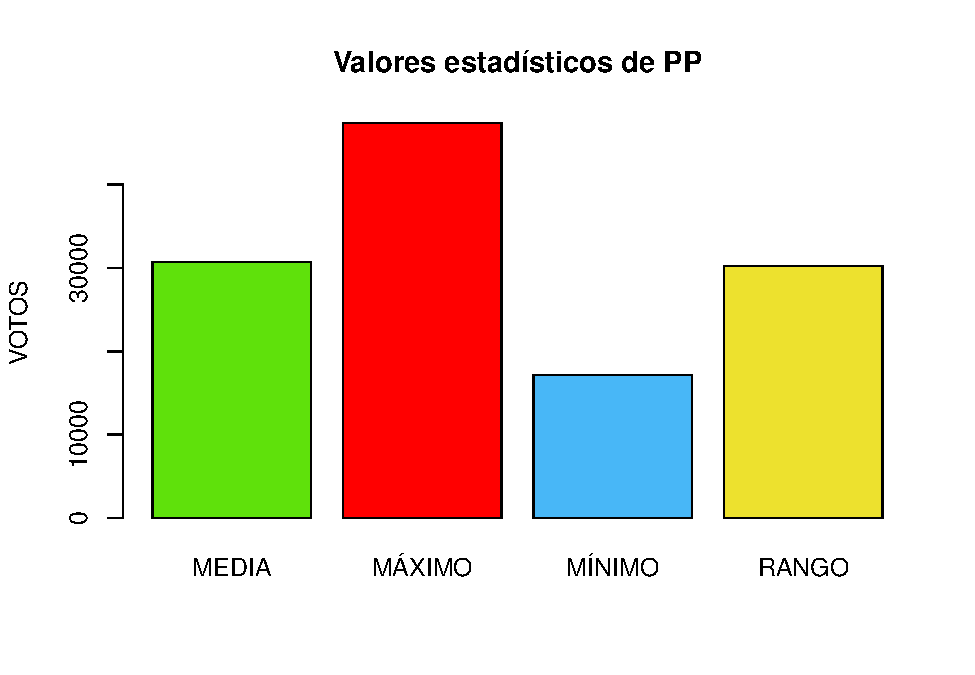
\includegraphics{SAFOR_files/figure-latex/6-1.pdf}

\begin{longtable}[]{@{}lr@{}}
\caption{ESTADÍSTICA SAFOR PP}\tabularnewline
\toprule\noalign{}
ESTADÍSTICA & VALORS \\
\midrule\noalign{}
\endfirsthead
\toprule\noalign{}
ESTADÍSTICA & VALORS \\
\midrule\noalign{}
\endhead
\bottomrule\noalign{}
\endlastfoot
MEDIA & 30729 \\
MÁXIMO & 47413 \\
MÍNIMO & 17142 \\
RANGO & 30271 \\
\end{longtable}

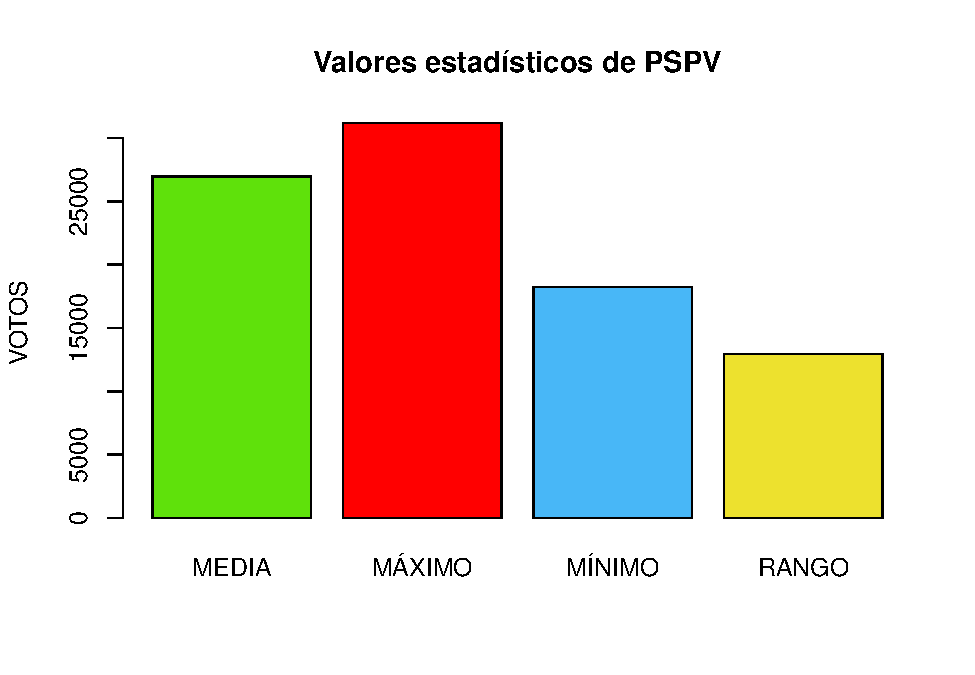
\includegraphics{SAFOR_files/figure-latex/6-2.pdf}

\begin{longtable}[]{@{}lr@{}}
\caption{ESTADÍSTICA SAFOR PSPV}\tabularnewline
\toprule\noalign{}
ESTADÍSTICA & VALORS \\
\midrule\noalign{}
\endfirsthead
\toprule\noalign{}
ESTADÍSTICA & VALORS \\
\midrule\noalign{}
\endhead
\bottomrule\noalign{}
\endlastfoot
MEDIA & 26985 \\
MÁXIMO & 31192 \\
MÍNIMO & 18226 \\
RANGO & 12966 \\
\end{longtable}

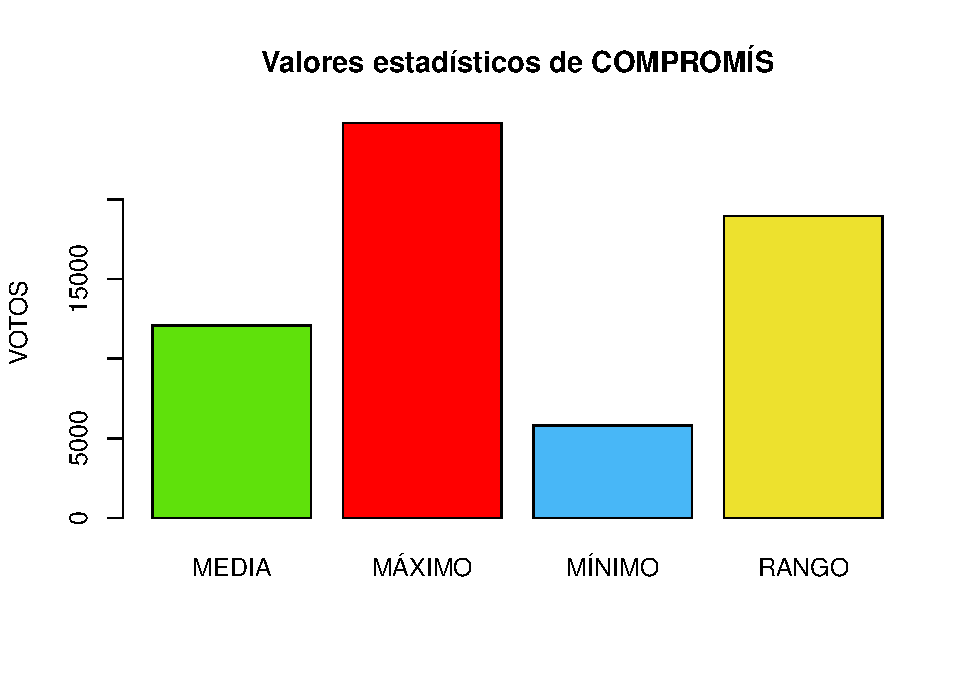
\includegraphics{SAFOR_files/figure-latex/6-3.pdf}

\begin{longtable}[]{@{}lr@{}}
\caption{ESTADÍSTICA SAFOR COMPROMÍS}\tabularnewline
\toprule\noalign{}
ESTADÍSTICA & VALORS \\
\midrule\noalign{}
\endfirsthead
\toprule\noalign{}
ESTADÍSTICA & VALORS \\
\midrule\noalign{}
\endhead
\bottomrule\noalign{}
\endlastfoot
MEDIA & 12094 \\
MÁXIMO & 24789 \\
MÍNIMO & 5823 \\
RANGO & 18966 \\
\end{longtable}

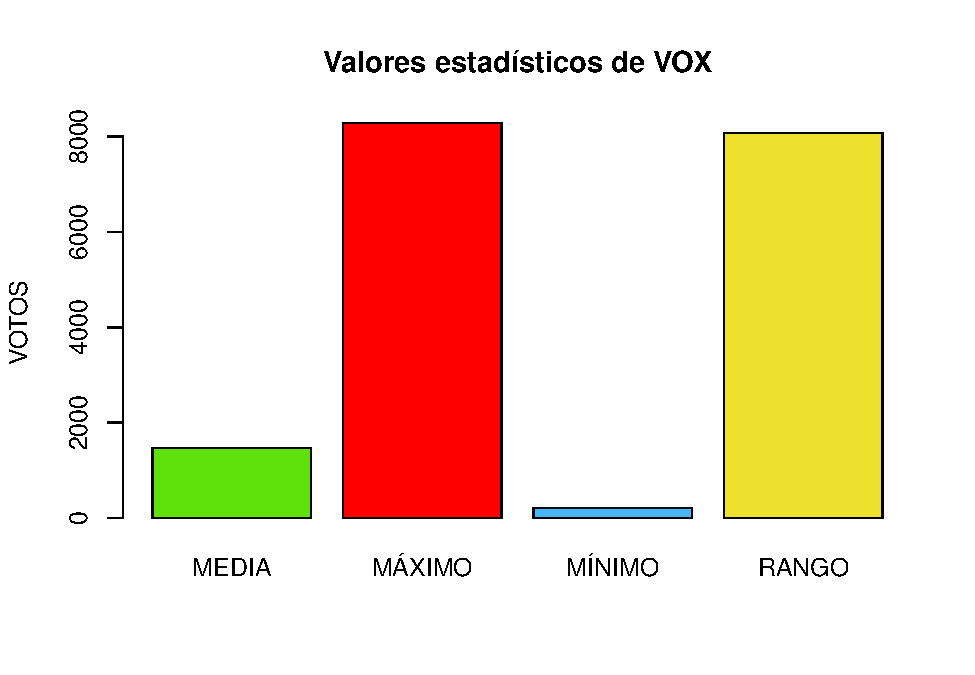
\includegraphics{SAFOR_files/figure-latex/6-4.pdf}

\begin{longtable}[]{@{}lr@{}}
\caption{ESTADÍSTICA SAFOR VOX}\tabularnewline
\toprule\noalign{}
ESTADÍSTICA & VALORS \\
\midrule\noalign{}
\endfirsthead
\toprule\noalign{}
ESTADÍSTICA & VALORS \\
\midrule\noalign{}
\endhead
\bottomrule\noalign{}
\endlastfoot
MEDIA & 1468 \\
MÁXIMO & 8282 \\
MÍNIMO & 207 \\
RANGO & 8075 \\
\end{longtable}

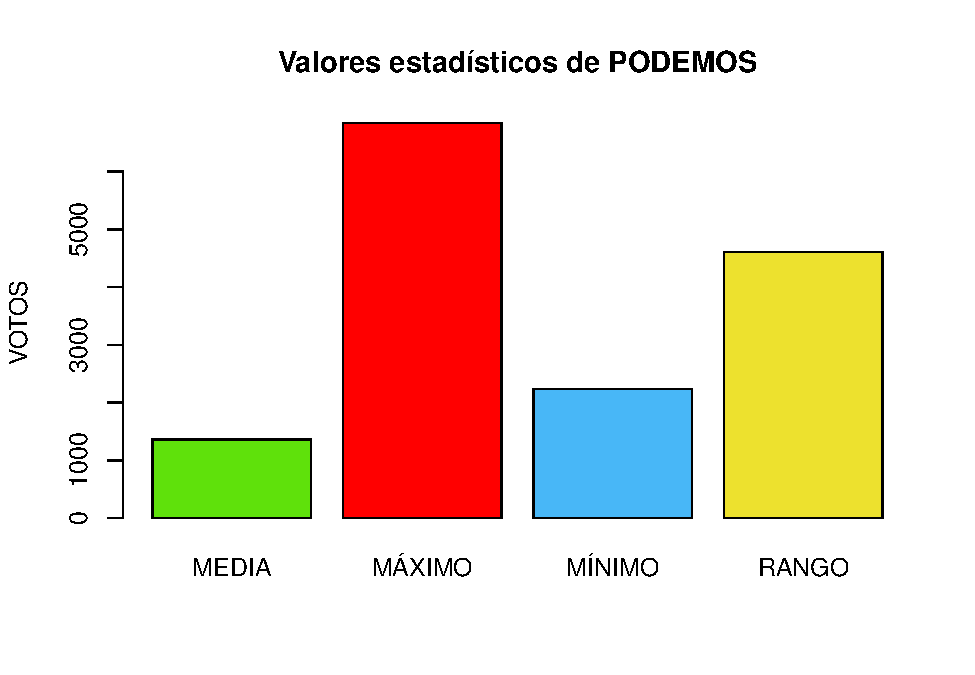
\includegraphics{SAFOR_files/figure-latex/6-5.pdf}

\begin{longtable}[]{@{}lr@{}}
\caption{ESTADÍSTICA SAFOR PODEMOS}\tabularnewline
\toprule\noalign{}
ESTADÍSTICA & VALORS \\
\midrule\noalign{}
\endfirsthead
\toprule\noalign{}
ESTADÍSTICA & VALORS \\
\midrule\noalign{}
\endhead
\bottomrule\noalign{}
\endlastfoot
MEDIA & 1363 \\
MÁXIMO & 6845 \\
MÍNIMO & 2234 \\
RANGO & 4611 \\
\end{longtable}

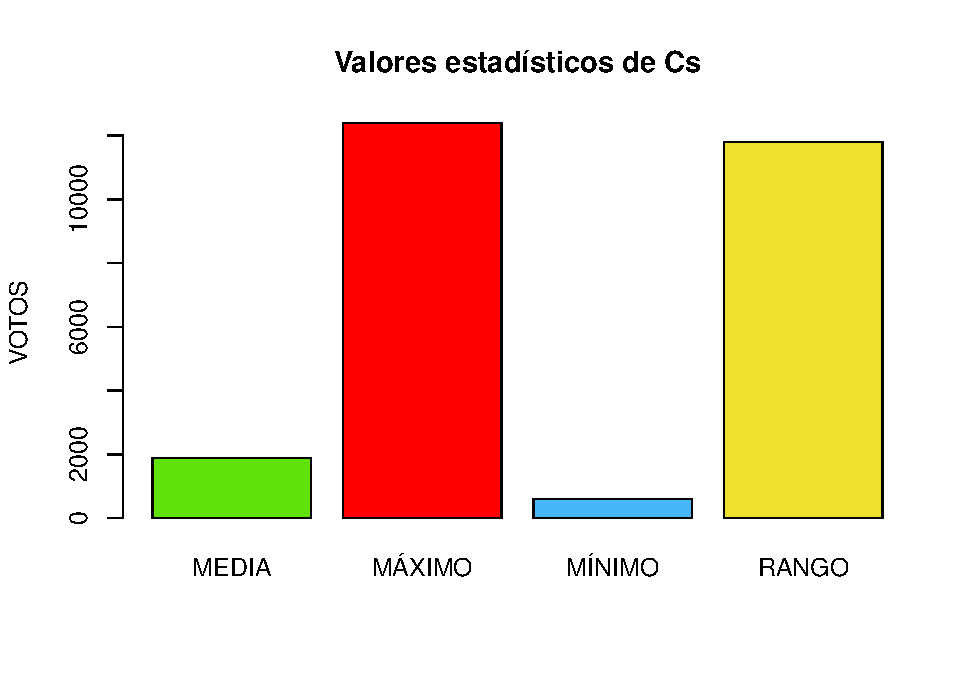
\includegraphics{SAFOR_files/figure-latex/6-6.pdf}

\begin{longtable}[]{@{}lr@{}}
\caption{ESTADÍSTICA SAFOR Cs}\tabularnewline
\toprule\noalign{}
ESTADÍSTICA & VALORS \\
\midrule\noalign{}
\endfirsthead
\toprule\noalign{}
ESTADÍSTICA & VALORS \\
\midrule\noalign{}
\endhead
\bottomrule\noalign{}
\endlastfoot
MEDIA & 1877 \\
MÁXIMO & 12394 \\
MÍNIMO & 591 \\
RANGO & 11803 \\
\end{longtable}

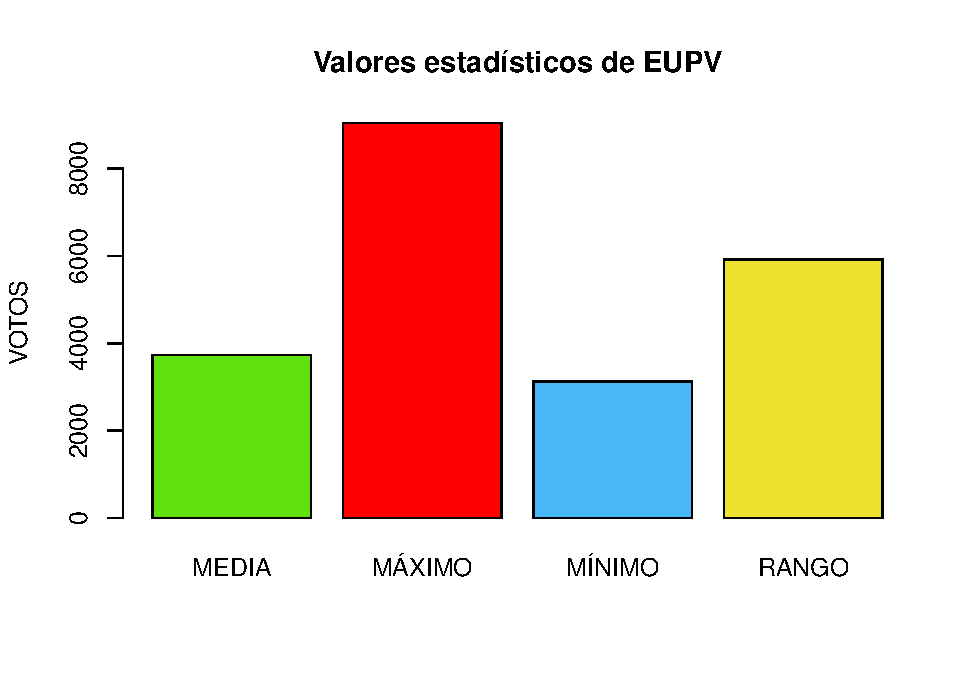
\includegraphics{SAFOR_files/figure-latex/6-7.pdf}

\begin{longtable}[]{@{}lr@{}}
\caption{ESTADÍSTICA SAFOR EUPV}\tabularnewline
\toprule\noalign{}
ESTADÍSTICA & VALORS \\
\midrule\noalign{}
\endfirsthead
\toprule\noalign{}
ESTADÍSTICA & VALORS \\
\midrule\noalign{}
\endhead
\bottomrule\noalign{}
\endlastfoot
MEDIA & 3732 \\
MÁXIMO & 9042 \\
MÍNIMO & 3129 \\
RANGO & 5913 \\
\end{longtable}

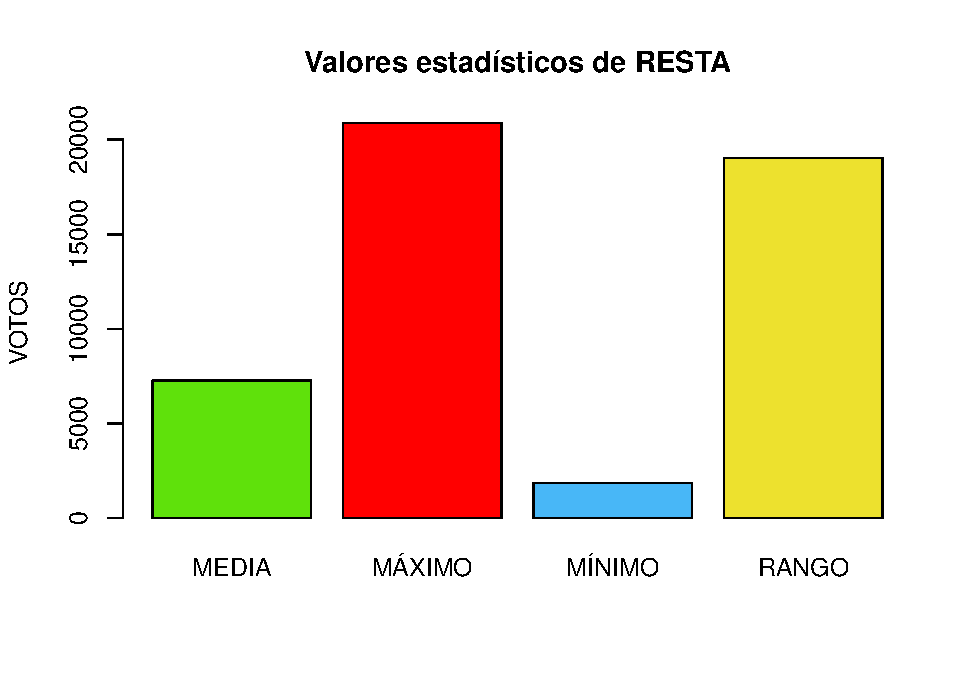
\includegraphics{SAFOR_files/figure-latex/6-8.pdf}

\begin{longtable}[]{@{}lr@{}}
\caption{ESTADÍSTICA SAFOR RESTA}\tabularnewline
\toprule\noalign{}
ESTADÍSTICA & VALORS \\
\midrule\noalign{}
\endfirsthead
\toprule\noalign{}
ESTADÍSTICA & VALORS \\
\midrule\noalign{}
\endhead
\bottomrule\noalign{}
\endlastfoot
MEDIA & 7255 \\
MÁXIMO & 20879 \\
MÍNIMO & 1859 \\
RANGO & 19020 \\
\end{longtable}

\end{document}
